\documentclass{standalone}
\usepackage{tikz}
\begin{document}
% Created by tikzDevice version 0.7.0 on 2015-03-19 12:54:23
% !TEX encoding = UTF-8 Unicode
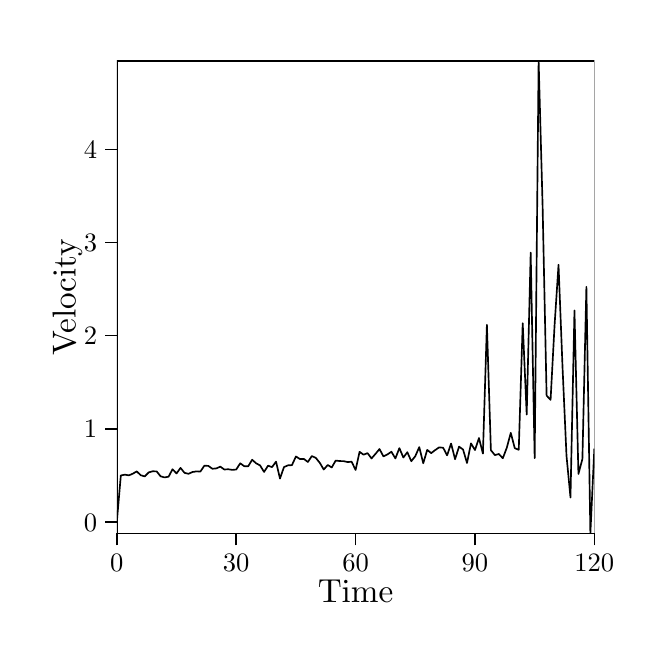
\begin{tikzpicture}[x=1pt,y=1pt]
\definecolor[named]{fillColor}{rgb}{1.00,1.00,1.00}
\path[use as bounding box,fill=fillColor,fill opacity=0.00] (0,0) rectangle (216.81,216.81);
\begin{scope}
\path[clip] (  0.00,  0.00) rectangle (216.81,216.81);
\definecolor[named]{drawColor}{rgb}{1.00,1.00,1.00}
\definecolor[named]{fillColor}{rgb}{1.00,1.00,1.00}

\path[draw=drawColor,line width= 0.6pt,line join=round,line cap=round,fill=fillColor] ( -0.00,  0.00) rectangle (216.81,216.81);
\end{scope}
\begin{scope}
\path[clip] ( 32.22, 34.03) rectangle (204.76,204.77);
\definecolor[named]{fillColor}{rgb}{1.00,1.00,1.00}

\path[fill=fillColor] ( 32.22, 34.03) rectangle (204.76,204.77);
\definecolor[named]{drawColor}{rgb}{0.00,0.00,0.00}

\path[draw=drawColor,line width= 0.6pt,line join=round] ( 32.22, 38.24) --
	( 33.66, 54.99) --
	( 35.10, 55.30) --
	( 36.54, 55.03) --
	( 37.97, 55.63) --
	( 39.41, 56.47) --
	( 40.85, 55.09) --
	( 42.29, 54.66) --
	( 43.72, 56.10) --
	( 45.16, 56.51) --
	( 46.60, 56.47) --
	( 48.04, 54.69) --
	( 49.48, 54.29) --
	( 50.91, 54.56) --
	( 52.35, 57.25) --
	( 53.79, 55.73) --
	( 55.23, 57.75) --
	( 56.67, 55.94) --
	( 58.10, 55.60) --
	( 59.54, 56.24) --
	( 60.98, 56.47) --
	( 62.42, 56.44) --
	( 63.85, 58.53) --
	( 65.29, 58.46) --
	( 66.73, 57.42) --
	( 68.17, 57.55) --
	( 69.61, 58.19) --
	( 71.04, 57.15) --
	( 72.48, 57.25) --
	( 73.92, 57.01) --
	( 75.36, 57.15) --
	( 76.80, 59.40) --
	( 78.23, 58.36) --
	( 79.67, 58.29) --
	( 81.11, 60.68) --
	( 82.55, 59.40) --
	( 83.98, 58.63) --
	( 85.42, 56.27) --
	( 86.86, 58.53) --
	( 88.30, 58.02) --
	( 89.74, 60.01) --
	( 91.17, 53.88) --
	( 92.61, 58.02) --
	( 94.05, 58.66) --
	( 95.49, 58.73) --
	( 96.93, 61.86) --
	( 98.36, 60.95) --
	( 99.80, 60.98) --
	(101.24, 59.87) --
	(102.68, 62.02) --
	(104.11, 61.35) --
	(105.55, 59.57) --
	(106.99, 57.15) --
	(108.43, 58.79) --
	(109.87, 57.89) --
	(111.30, 60.38) --
	(112.74, 60.21) --
	(114.18, 60.17) --
	(115.62, 59.84) --
	(117.06, 59.97) --
	(118.49, 56.98) --
	(119.93, 63.54) --
	(121.37, 62.50) --
	(122.81, 63.07) --
	(124.24, 61.15) --
	(125.68, 62.80) --
	(127.12, 64.55) --
	(128.56, 61.89) --
	(130.00, 62.60) --
	(131.43, 63.57) --
	(132.87, 61.15) --
	(134.31, 64.88) --
	(135.75, 61.49) --
	(137.19, 63.40) --
	(138.62, 60.14) --
	(140.06, 61.96) --
	(141.50, 65.25) --
	(142.94, 59.40) --
	(144.37, 64.24) --
	(145.81, 63.07) --
	(147.25, 64.18) --
	(148.69, 65.15) --
	(150.13, 65.02) --
	(151.56, 62.26) --
	(153.00, 66.53) --
	(154.44, 60.88) --
	(155.88, 65.42) --
	(157.32, 64.38) --
	(158.75, 59.50) --
	(160.19, 66.60) --
	(161.63, 64.18) --
	(163.07, 68.52) --
	(164.50, 62.90) --
	(165.94,109.46) --
	(167.38, 64.14) --
	(168.82, 62.36) --
	(170.26, 62.76) --
	(171.69, 61.22) --
	(173.13, 65.02) --
	(174.57, 70.40) --
	(176.01, 64.85) --
	(177.45, 64.28) --
	(178.88,110.03) --
	(180.32, 76.99) --
	(181.76,135.53) --
	(183.20, 61.25) --
	(184.63,204.77) --
	(186.07,152.28) --
	(187.51, 83.86) --
	(188.95, 82.31) --
	(190.39,109.26) --
	(191.82,131.12) --
	(193.26, 94.29) --
	(194.70, 62.13) --
	(196.14, 47.05) --
	(197.58,114.61) --
	(199.01, 55.53) --
	(200.45, 60.95) --
	(201.89,123.18) --
	(203.33, 34.03) --
	(204.76, 64.72);

\path[draw=drawColor,line width= 0.6pt,line join=round,line cap=round] ( 32.22, 34.03) rectangle (204.76,204.77);
\end{scope}
\begin{scope}
\path[clip] (  0.00,  0.00) rectangle (216.81,216.81);
\definecolor[named]{drawColor}{rgb}{0.00,0.00,0.00}

\node[text=drawColor,anchor=base east,inner sep=0pt, outer sep=0pt, scale=  0.96] at ( 25.11, 34.93) {0};

\node[text=drawColor,anchor=base east,inner sep=0pt, outer sep=0pt, scale=  0.96] at ( 25.11, 68.58) {1};

\node[text=drawColor,anchor=base east,inner sep=0pt, outer sep=0pt, scale=  0.96] at ( 25.11,102.22) {2};

\node[text=drawColor,anchor=base east,inner sep=0pt, outer sep=0pt, scale=  0.96] at ( 25.11,135.86) {3};

\node[text=drawColor,anchor=base east,inner sep=0pt, outer sep=0pt, scale=  0.96] at ( 25.11,169.50) {4};
\end{scope}
\begin{scope}
\path[clip] (  0.00,  0.00) rectangle (216.81,216.81);
\definecolor[named]{drawColor}{rgb}{0.00,0.00,0.00}

\path[draw=drawColor,line width= 0.6pt,line join=round] ( 27.95, 38.24) --
	( 32.22, 38.24);

\path[draw=drawColor,line width= 0.6pt,line join=round] ( 27.95, 71.88) --
	( 32.22, 71.88);

\path[draw=drawColor,line width= 0.6pt,line join=round] ( 27.95,105.52) --
	( 32.22,105.52);

\path[draw=drawColor,line width= 0.6pt,line join=round] ( 27.95,139.16) --
	( 32.22,139.16);

\path[draw=drawColor,line width= 0.6pt,line join=round] ( 27.95,172.81) --
	( 32.22,172.81);
\end{scope}
\begin{scope}
\path[clip] (  0.00,  0.00) rectangle (216.81,216.81);
\definecolor[named]{drawColor}{rgb}{0.00,0.00,0.00}

\path[draw=drawColor,line width= 0.6pt,line join=round] ( 32.22, 29.77) --
	( 32.22, 34.03);

\path[draw=drawColor,line width= 0.6pt,line join=round] ( 75.36, 29.77) --
	( 75.36, 34.03);

\path[draw=drawColor,line width= 0.6pt,line join=round] (118.49, 29.77) --
	(118.49, 34.03);

\path[draw=drawColor,line width= 0.6pt,line join=round] (161.63, 29.77) --
	(161.63, 34.03);

\path[draw=drawColor,line width= 0.6pt,line join=round] (204.76, 29.77) --
	(204.76, 34.03);
\end{scope}
\begin{scope}
\path[clip] (  0.00,  0.00) rectangle (216.81,216.81);
\definecolor[named]{drawColor}{rgb}{0.00,0.00,0.00}

\node[text=drawColor,anchor=base,inner sep=0pt, outer sep=0pt, scale=  0.96] at ( 32.22, 20.31) {0};

\node[text=drawColor,anchor=base,inner sep=0pt, outer sep=0pt, scale=  0.96] at ( 75.36, 20.31) {30};

\node[text=drawColor,anchor=base,inner sep=0pt, outer sep=0pt, scale=  0.96] at (118.49, 20.31) {60};

\node[text=drawColor,anchor=base,inner sep=0pt, outer sep=0pt, scale=  0.96] at (161.63, 20.31) {90};

\node[text=drawColor,anchor=base,inner sep=0pt, outer sep=0pt, scale=  0.96] at (204.76, 20.31) {120};
\end{scope}
\begin{scope}
\path[clip] (  0.00,  0.00) rectangle (216.81,216.81);
\definecolor[named]{drawColor}{rgb}{0.00,0.00,0.00}

\node[text=drawColor,anchor=base,inner sep=0pt, outer sep=0pt, scale=  1.20] at (118.49,  9.03) {Time};
\end{scope}
\begin{scope}
\path[clip] (  0.00,  0.00) rectangle (216.81,216.81);
\definecolor[named]{drawColor}{rgb}{0.00,0.00,0.00}

\node[text=drawColor,rotate= 90.00,anchor=base,inner sep=0pt, outer sep=0pt, scale=  1.20] at ( 17.30,119.40) {Velocity};
\end{scope}
\end{tikzpicture}
\end{document}
